\chapter{A Social Contract for Cyberspace}

\section{Introduction}
This chapter addresses a critical
weakness in the whole concept on which the dissertation is based. It
addresses a crucial issue on which they all depend: ``How can stakeholders
agree with each other about what is allowed in each other's policies?''

In our world, the ethics of humans including business rules can be different from one to another,
without the necessity for conflict. There are, probably, some ethical
principles that are ``universal'', i.e. we all share them. Respect for life, for property, are examples of values which {\em most} citizens respect. But there are other values (ethics, or agreed principles of behaviour in general) 
that are not universal. The fact that human values vary from person to person does not obviate
the need to incorporate human and ethical values (and principles
of operation in general) into software. According to this dissertation's point of view, the
key to achieving this goal, without forcing all users to adopt ethical
principles that they don't agree with, is to seek agreement only on a
core set of ethical principles: the social contract.

It might appear that the proposed social contract in this chapter is not a
technical concept but rather, merely, an appeal to the good behaviour of
citizens of cyberspace. However, the authors in \cite{sheniar2021social}
expect that technical means for enforcing policies will become more
widespread, leading to \iffalse an increasingly rigorous, and technical, role
for the social contract\fi an increasingly rigorous, and technical, role for the social contract that is proposed in this chapter. 







%\section{Introduction2}

\iffalse
As the Internet and its residents, human and otherwise, grow in
expressiveness, creativity, and energy, it seems inevitable that
there will also emerge a growing need for, and development of, {\em
regulation}. To some, this may seem like a betrayal of the original ideals
of the Internet.  On the other hand, if such regulation is neglected,
as we argue it has been up to now, the regulations imposed by nation
states, corporations, and other stakeholders, might cast an unnecessary
and unwanted shadow on cyberspace.
\fi
In \cite{sheniar2021social}, we argued that cyberspace needs a {\em
social contract}\index{social contract}, with its entities (individual users, organisations,
devices, and service providers), and we went on to set out criteria
for such a social contract, we reviewed the issues which it addresses,
we proposed a draft contract, and, finally, we reviewed how well this
draft contract addresses those issues.


The main contribution of this chapter is to demonstrate the need for a
social contract for cyberspace (and the Internet), i.e. a declaration
of responsibilities and rights of all members of cyberspace, and also
to propose a draft of such a social contract.
\iffalse
Any such social contract will need to enable and manage the stakeholders'
policies, rather than enforce them. Details of protocols, services, and
protections will still need to be the responsibility of entities that
participate and contribute to cyberspace. The task before this chapter
is not to design such safeguards and mechanisms, but rather to enable
their free and effective development, evolution, and deployment.
\fi
In the remainder of this introductory section, we review the initiatives
in the recent history of cyberspace that overlap most closely with the
work of the present chapter and then outline the rest of the chapter.

\subsection{The Structure of Cyberspace}\label{strcofcyb}

Cyberspace\index{cyberspace} is a collection of entities (agents,
devices, servers, and more) Figure \ref{policiesfig}. Each entity has
a {\em policy}. The policy protects the entity where it is located, and
also declares conditions it commits to, for other agents or devices. A
policy is a statement of obligations and conditions.


\begin{figure}
	\centering
		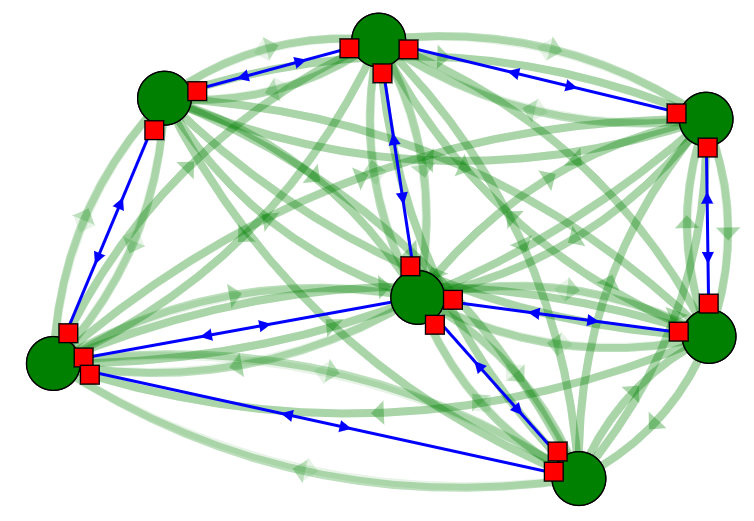
\includegraphics[width=8cm]{figures/policies.png}
\caption{policies}
\label{policiesfig}
\end{figure}

According to this dissertation's point of view, the entities can be classified into, the services, and their stakeholders as shown in Figure \ref{Cyberspacefig}. Stakeholders can set their own policies regarding the services they engage with. These policies are used to achieve key (essential) stakeholder objectives. The stakeholders should be able to work together effectively although they have different objectives.
\begin{figure}
	\centering
		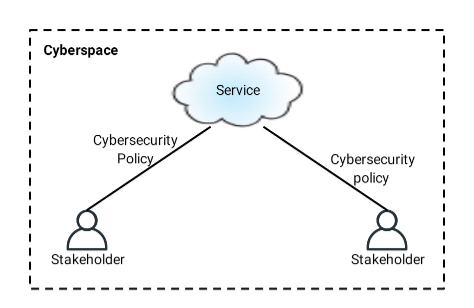
\includegraphics[width=8cm]{figures/Cyberspace.png}
\caption{Cyberspace}
\label{Cyberspacefig}
\end{figure}
 However, before we can even state these objectives, it is essential to gain agreement between all the parties affected. In other words, to gain agreement to a "contract". Without such a contract, cybersecurity is not possible, because it has no clear goal. But, with such a contract, there is a relatively obvious, systematic process to achieve cybersecurity. 
 
We must design, develop and implement software that enforces the social contract, and ensure that everyone installs this software and uses only this software in the course of their interaction (Like the Uber App in Subsection \ref{gigsol}).


\subsection{The Social Contract}
Social contracts are considered a necessity and an essential factor for the well-being of societies because they regulate their members' relations within those societies \cite{Leviathan}. As social computing \cite{parameswaran2007social}, cyberspace may need a social contract which declares the responsibilities and rights of all members of cyberspace. Any such social contract will need to enable and manage the stakeholders' policies, rather than enforce them. Details of these policies will still need to be the responsibility of stakeholders that participate and contribute to cyberspace. However, the task of this social contract is to enable free and effective development, evolution, and deployment of these policies

\iffalse
The concept of a social contract appears to have originated in ancient
Greece, with the sophist philosophers and Epicurus. Plato has been
found to both explain the concept of the social contract and to reject
it (as a foundation for justice)  \cite{Plato5} .
%\cite{Plato5,PlatoR}. 
The Magna Carta was a legal agreement by the English King John
guaranteeing certain rights and protections to the English barons, 
declared in 1215, and revised and redeclared
multiple times since then. Although originally it protected only barons,
its extension to all free men and women appears to have been perceived
as a logical necessity in subsequent years.

\iffalse
The modern
resurgence of the social contract is associated with the philosophers
Hobbes \cite{Leviathan}, circa 1650, Locke, Voltaire, and Rousseau and also with great
political changes in England, the United States, and France in which
individuals outside the privileged classes, and large communities of
such individuals made major contributions toward the theoretical
and practical implementation of a social contract in England, the United
States, and France \cite{Goodall}.
\fi

According to Hobbes \cite{Leviathan}, without a social contract, life is subject to
\begin{quote}\em
continual fear, and danger of violent death; and the life of man, solitary, poor, nasty, brutish, and short.
\end{quote}
However, a social contract between the citizens of a society enables them to co-operate
effectively, to achieve a better life without the need for constant fear.

The Internet has made computing social \cite{parameswaran2007social}. In
turn, the Internet and the cyberspace based on it, is susceptible to
a number of social ills that may befall any society, such as constant
harassment, belligerent attacks on property, that is, cyberattacks,
and invasions of privacy which seriously compromise the benefits for our
social, educational, and commercial lives. Are these issues (which are
surveyed in more detail in Section \ref{issues}) due to the absence
of a social contract?

Although the Declaration of Independence of the United States of America stated
\begin{quote}\em
We hold these truths to be self-evident, that all men are created equal,
that they are endowed by their Creator with certain unalienable Rights,
that among these are Life, Liberty and the pursuit of Happiness,
\end{quote}
slavery remained a part of the society which subscribed to this social contract
for another 80 years. 
%
Social contracts have been adopted in many modern nations, and in many cases they
appear to provide a good foundation for civil society, providing safety, wide-ranging 
freedom, with a high standard of living. Attempts to formulate an {\em international}
social contract, have been at best partially successful. There is an international court
of justice, but many nations do not accept its jurisdiction \cite{Robertson}.

\fi
\subsection{Service Level Agreements}\label{slasec1}

Currently, users of the Internet are likely to have agreed to a {\em service level
agreement} with their Internet provider \cite{RFCs}. Functionally, this is similar to a social
contract, the main difference being that the roles envisaged in such agreements
are quite asymmetrical -- the provider has certain obligations, and so does the consumer
of their services, but these obligations are usually quite different. This is discussed
in more detail in \S\ref{slasec}.

\subsection{Standards}\label{standards}

The current standards for the Internet and its services and devices 
are set and developed by multiple standards organisations \cite{ietf} %,ITU,IEEE,ETSI,ISO},
and also national governments. In \cite{sheniar2021social} we argued that a {\em social contract} 
(like a constitution and a bill or rights) is needed between
these organisations, and the entities which use the Internet to communicate.

\subsection{Web 2.0, the Semantic Web, or Web 3.0}\label{web2}

Web 2.0 \cite{tim2005web} is a name used to explore and to some extent explain
the social network applications and development that has emerged from 
and in turn influenced the world-wide web.

% \subsection{The Semantic Web, or Web 3.0}\label{web3}

Web 3.0, or the {\em semantic web} \cite{berners2001semantic} provides a
systematic standardized technology for cross-referencing, from document
to document, and to specific parts of documents.  Furthermore, by this
means, and by agreed conventions for how key information is stored,
the agents which operate in user and network devices are able to extract
not just data but also the {\em meaning} of this data from the documents
they have access to.  This is achieved, it is claimed, by using XML to
structure data, and RDF \cite{rdf} to describe its meaning. In this way,
the quality and effectiveness of the services provided by the Internet
will be transformed, according to the proponents of the Semantic Web.

\subsection{The dark side}

Some of the developments anticipated in the semantic web concept have come to pass. However, the problems listed below, in Section \ref{issues}, undermine somewhat the idea that facilitating reference, access, and meaningful interpretation of web data, will enable good sense to triumph in cyberspace. With the convenience and intelligence offered by electronic agents inhabiting the web, and the world of apps, a crowd of unwanted denizens focused on criminality, exploitation, fraud, and chaos have taken the opportunities (of which there are many) to join us in cyberspace.

It seems that we need more than a universal API for access to the meaning in the Internet and its contents to ensure that good sense has enough advantage over greed, competitive advantage, and, in general, the forces of human frailty. We must assume that whenever there is an opportunity for error, fraud, deception, or intimidation, it will be exploited. We need to actively defend against criminality, greed, parochialism, and chaos.

\subsection{Outline of the chapter}

In Section \ref{criteria}, criteria for a social contract for cyberspace are outlined, in Section \ref{issues}, fourteen serious and ongoing ethical or security issues in the Internet and cyberspace are reviewed, in Section \ref{necessity}, the questions of whether a social contract is really necessary, whether it is possible, and also whether in a sense it already exists are explored, in Section \ref{proposedsc} a draft social contract is outlined, including a review of how this draft social contract succeeds in addressing the issues presented in Section \ref{issues}, and, finally, in Section \ref{conc} conclusions are presented.

\section{Criteria for a Social Contract}\label{criteria}

\begin{enumerate}[C-1.]

\item\label{canachieve} Any entity using the Internet is able to achieve its goals (including adequate cyber-security), by setting and enforcing its public policy, so long as this policy is consistent with the social contract for cyberspace.

\item\label{sameforall} The obligations and rights {\em provided by the Internet social contract} are the same for all entities.
\end{enumerate}

These criteria are natural and yet quite powerful, and we shall see that their implications are surprisingly effective. Because the ethical assumptions made by members of cyberspace are currently not explicit, it is not possible at present to explain these criteria by reference to existing work.

The first of these criteria merely says that all entities are entitled to {\em be able} to engage securely with the Internet, so long as they do not seek to transgress its norms.

The second criterion is the natural condition that any rules should apply uniformly to all participants. Note that the specific policies adopted by, and agreed to, by entities in the course of providing and using services are not expected to be the same for everyone.

\section{Current Ethical and Cybersecurity Issues}\label{issues}

Cyberspace is currently burdened by many chronic and serious issues which frequently cause harm. In this section, the problems are presented. Here follows a classified survey of such issues, including some accounts of their particular features in a form that is relevant to their subsequent discussion, in \S \ref{address} in which all these issues are solved.

\subsection{Cyber-Attack}\label{cybattk}

\subsubsection*{Issue I-\ref{cyberwar}. {Cyber-warfare}}\label{cyberwarsol}
%
Most developed nations currently posess a national agency
engaged in defence, {\em and attack}, through the Internet,
against the cyberspace services and resources of rival nations.
These agencies seek to gain access and defend against
access by others to public and secret information
about technology (especially military technology),
politics and commerce. 
Such agencies also frequently engage in {\em disruption} of the same systems. Probably
the most famous example of such activity is the development
and deployment of the {\em Stuxnet} virus (actually called the 
{\em Olympic Games virus} by its developers)  \cite{kushner2013real,langner2011stuxnet} .


% \subsection{A Case Study -- Stuxnet}

% \subsubsection{Background}

Stuxnet is a very sophisticated malware program designed to  attack  industrial
cyber-physical systems  \cite{karnouskos2011stuxnet}. It targetted
a specific industrial laboratory -- the Natanz uranium enrichment plant \cite{karnouskos2011stuxnet}.
The challenge was that this plant is completely isolated from the Internet
\cite{chen2010stuxnet}.  Stuxnet is designed to be autonomous \cite{kushner2013real}. 
It used four zero day exploits \cite{chen2010stuxnet}, which made it difficult to detect
or prevent using the security technologies available at the time.

The development and deployment of Stuxnet has been noted
as a major backward step in the standard of behaviour that might
be expected in cyberspace. Any agreement, technology, or architecture
that is able to prevent recurrences of this behaviour will
be universally applauded, but it is unlikely that any nation will
adopt measures which do that unless they can be {\em certain}
that these measures apply to {\em all} entities equally.

Cyberwarfare is the most critical of all the issues we consider, 
and also has the greatest natural association with the question of regulating
good behaviour. If a social contract can help us with this issue,
it deserves our strong support.


% \subsection* {Example -- Stuxnet}

\subsubsection*{Issue I-\ref{viruses}. {Viruses}}\label{virusessol}
%
A virus is an item of software that installs itself, or is installed
(usually without the conscious knowledge of the user),
and then runs on a user's computer, or device, or on a server, and 
takes actions unwanted by the user, such as stealing, corrupting,
or encyrpting data.

Viruses are developed by state actors, such as the agencies
referred to in I-\ref{cyberwar}, by criminal organisations, working
to generate income by extortion or fraud, and by individuals.

\subsubsection*{Issue I-\ref{identitytheft}. {Identity Theft}}\label{identitytheftsol}
%
The simplest form of identity theft is for an attacker to find, discover,
or guess another user's password, and then use it for services
they are not entitled to. 

The more complex form of identity theft is where an attacker gathers
information about a target person, mostly or all from public
sites, and then uses this information to take control of resources
(bank accounts, phone accounts, etc) of the victim. 

\subsubsection*{Issue I-\ref{fraud}. {Fraud}}\label{fraudsol}
%
A simple example of fraud which is currently feasible in cyberspace is
the unintended release to, or alteration by, a third party, of credit card or financial account
credentials. For example, the account into which an employee's salary is to
be paid.

\subsubsection*{Issue I-\ref{phishing}. {Phishing}}\label{phishingsol}
%
Phishing is the practice of tricking the target into an unintended action
by sending them an email (or message) which appears to be from a trusted
source, or is of a frequently recieved and therefore expected form, which
then triggers a semi-automatic response which has, in this instance, an
unexpected (and probably secret) side-effect, such as installing a virus.

\subsection{Exploitation}\label{exploitationsec}
\subsubsection*{Issue I-\ref{appstore}. {App-stores and Software Repositories}}\label{appstoresol}
%
App stores such as Apple's App Store, and the Play Store on Android smart phones
play an important role in the protection of users from attack. Software
provided in an App Store is checked by professional staff. In addition, all apps
are required to declare a policy which is then enforced by the smart-phone
operating system. This much is entirely consistent with the social contract
proposed in Section \ref{proposedsc}.

However, this method for distributing and validating smart phone software
directly contradicts Criterion C-\ref{sameforall}. Operating system vendors
are adopting a highly asymmetical role relative to users in this approach
to protection of users. 

\subsubsection*{Issue I-\ref{gig}. {The Gig-economy (Uber et al)}}\label{gigsol}
%
Along with streamlining and increasing flexibility, repackaging services to handle
service description and payment details by means of a smart-phone app, 
the so-called Gig-economy, has frequently had the side-effect of
disempowering many of those involved in providing the service (the workers).

\subsubsection*{Issue I-\ref{monop}. {Monopolistic behaviour}}\label{monopsol}
%
Monopolistic behaviour in the information, communication and computer industry
has been prevalent virtually from the start. It has been addressed, in the
telecommunications industry, by anti-trust legislation in the United States
and similar legislative changes were adopted afterwards in many other countries.
This intervention of the legal and legislative arms, of the U.S. and other
governments, was viewed by many, at the time, as unwarranted meddling. However,
with the perspective provided by 40 years of history, it appears to have been
justified, and highly successful.

It was, nevertheless, highly disruptive, and if there are means to avoid
the necessity for intervention by politicians and judges, it will be preferable.


\subsection{Social networking}\label{evolution}

\subsubsection*{Issue I-\ref{exileissue}. {Exile or censorship (of social network users)}}\label{exile}
%
The policy of banning certain users from access to Facebook, twitter, or another social
media application because of their perceived promulgation of false or dangerous beliefs
is likely to be contentious \cite{parameswaran2007social}. Whether certain beliefs are false, or dangerous, is unlikely
to be ascertained with universal agreement by any board of review no matter how carefully
chosen.

\subsubsection*{Issue I-\ref{Fakenews}. {Fake news}}\label{disinfsol}
%
Fake news is the name given to false information promoted as
genuine, either in error, or knowingly because the promoter wishes
other cyberspace citizens to be misinformed  \cite{carson2021fighting}.
The widespread availability of digital sources of information, including
digital signatures to verify authenticity, is reducing the scope for
deliberate disinformation, but for the moment it remains a problem.

\subsubsection*{Issue I-\ref{bullying}. {Cyber-bullying}}\label{bullyingsol}
%
Bullying is a phenomenon of concern that goes beyond just the forms
appearing in cyberspace. However, social networking, and cyberspace in general,
can have the effect of intensifying such bullying to unprecedented, unacceptable, levels.


\subsubsection*{Issue I-\ref{minors}. {Protection of minors}}\label{minorssol}
%
Before the age of approximately 18, citizens are not regarded as competent
to indendently engage in society. Up to approximately this age, they
require the supervision and protection of a guardian, usually but not always 
a parent. For example, children below this age engaged in play or exercise in a swimming
pool {\em must} be accompanied by a responsible adult. Society includes 
risks of many sorts, and so, such supervision and responsibility is
required almost constantly for non-adults. Cyberspace, as a part of society which
reflects most of its components (good and bad), is also a domain
in which supervision and guidance is required.

% \item\label{disinf}{\bf User access control and control of disinformation}

\subsubsection*{Issue I-\ref{locality}. {Local cultural traditions (locality, community)}}\label{localitysol}
%
Cultural, social, legal, and ethical traditions vary from place to place, and from community
to community. Although the sharing of a medium of exchange for services and information might
be expected to introduce greater homogeneity in such traditions and conventions, it is not
appropriate to empower or enable such a process of convergence. On the contrary, it seems
more reasonable that local traditions, if they are genuinely supported by a community, should
be enabled and preserved.

Is it feasible to define and adopt a common social contract which is also neutral in its
impact on locally distinct cultural traditions?

\subsection{Technical Development and Evolution}\label{evolution}

\iffalse
\item\label{BGPDNS}{\bf Routing Information and Domain Name Services.}
%
The original routing information protocols and domain name service protocols
assumed that servers could be trusted to provide accurate information, did 
not require authentication, and the information they exchanged could be
visible to other devices without risk. These protocols have since been
updated to ``secure'' versions, primarily by the addition of authentication
and encryption, however the original versions are still widely used.
\fi

\subsubsection*{Issue I-\ref{standardsissue}. {Standards Evolution}}\label{standardssol}
%
The majority of Internet standards take the form of RFCs, \cite{RFCs}
which are developed under the supervision of the IETF \cite{ietf}.
These standards can be of critical importance to the technical and
financial success of the companies providing hardware, software, and
services supporting cyberspace, employees of whom are the main particpants
in the committees which develop new standards. Consequently there is a considerable
risk of conflicts of interest in the development process.


\section{Necessity and Existence}\label{necessity}

Is it perhaps possible to achieve the criteria for a social contract for cyberspace
without any such agreement being formed? Or, on the contrary, can we show that
these very reasonable objectives are unattainable without such an agreement?
Is a social contract which addresses any of these issues actually feasible
(see \S\ref{address})?

Let us consider whether a social contract is possible, 
and if it is possible, how might it be enforced.
\iffalse
In this section, we explore these questions, in a general context; once
a draft social contract has been formulated, we shall review the issues
again by reference to the previous list of issues.\fi

\subsection{Do the existing standards form a social contract for cyberspace?}

The main Internet standards are known as RFCs (Request for Comments) \cite{RFCs}.
There are currently more than 9000 RFCs. These documents provide detailed
technical descriptions of all the main protocols and algorithms used to
implement the Internet. The primary form taken by these documents is a description
of how certain types of communication {\em must}, or in some cases, {\em may be} 
formed (some features and procedures are optional).

A scan of the RFC collection using terms with likely association with a
contract for cyberspace shows that even when these terms are used it
is in the context of organization or technical specification but not
in the context of implementing or discussing a social contract as proposed in this 
paper. The search terms used in this scan of the RFCs were: {\tt ethics,
society, social, moral, morals, human, humane, governance, organization,
contract, service, SLA, agreement, privacy}.

Standards other than RFCs, which are issued by the other standards bodies \cite{ITU,IEEE,ETSI,ISO}
(and perhaps some other organisations) also play an important role in defining and
regulating the Internet.

The funding for these standards bodies comes from governments, commercial organisations,
and private individuals (for example, members of the IEEE). In most cases committees of
qualified professionals are formed which meet from time to time, discussing
issues and details of proposed standards, and then formulating original drafts and 
subsequently revisions of standards. The time required by individuals in such committees 
is a significant cost, which in most cases is borne by the organisation from which
the individual comes.

\subsection{Do service level agreements form a social contract?}\label{slasec}

Existing service level agreements tend to be designed primarily
to provide legal protection against complaints from customers. The widespread (almost
universal) existence of service level agreements acknowledges their logical
necessity. However, they are rarely written in a manner which fully respects
the reciprocity of the relationship between service provider and client, 
and there is often no discussion of enforcement.



\subsection{Is a cyberspace social contract necessary?}

Political social contracts {\em emerged}  
in the form of the Assize of Clarendon (1166), the Magna Carta (1215),  
``An Agreement of the People'' (1647 -- during the English civil war), the U.S.
Declaration of independence (1776), and the Declaration of the Rights of Man 
and of the Citizen (France, 1789), and, finally, the United Nations declared the {\em Universal Declaration
of Human Rights} in 1948 \cite{unhdr} with 48 of the 58 nations voting for it.
The difference between an ``emerging'' social contract, and one which is
explicit, and enforcable is important.  Conscious awareness of 
enforcability will enhance its effectiveness.
 Just as, in many societies, a social contract has been found to be beneficial for the prosperity and well-being of citizens, a social contract can enable the prosperity and well-being of the entities which inhabit cyberspace.

\subsection{Is a social contract possible?}

The usefulness of the type of social contract considered in this paper
depends to a significant degree on its enforcability. We shall see, in \S\ref{gigsol}
in the case of Issue I-\ref{gig},
that some policies are readily and naturally enforcible. Enforcibility also
appears to be feasible for many other policies, e.g. I-\ref{fraud}.
Before it can be implemented as a standard, it will be necessary
for the community of Internet practitioners, academics, and users to debate
the matter. If there is sufficient support, progression to a standard would then
proceed according to the usual process for RFCs.

\subsection{Enforcement}\label{enforcement}

Traditionally, the legal framework of a nation state, which is the main substance, 
in mass, of the social contract adopted therein, is enforced by a legal system of 
police, courts, lawyers, judges and juries. This system is empowered to impose
imprisonment, exile (in the case of non-citizens), and fines.

In the case of cyberspace such remedies are rare, but not unknown. Imprisonment is
highly unlikely to be used as a remedy     \cite{parameswaran2007social}, but exile (in the sense of preventing
access to certain services) has become a preferred remedy in some contexts (for example,
President Trump's exile from twitter).

A more universally applicable enforcement mechanism, however, is probably the
maintenance of public, incontrovertible records of past actions. The most prominent
example of this currently is the block-chain system adopted in Bitcoin, and 
other digital currencies. Block-chains that provide public incontrovertible
records of actions have also been adopted for other purposes, for example records
of share transactions.

A public, accurate, incontrovertible record of actions serves more or less directly
as an enforcement mechanism in the case of the social contract proposed in
Section \ref{proposedsc} because each entity which provides services is required
to provide a {\em public policy}. This public policy is not merely a collection
of words, sentences, and paragraphs, which users acknowledge, but is required
to be formally precise, as explained in \S\ref{formalpolicies}. Consequently, whenever
an entity takes an action which is not consistent with their policy, if there
is a sufficiently detailed record of actions, which is public, any actions taken
which are not rigorously in accordance with the public policy will be detected.
An entity which takes an action inconsistent with its public policy will therefore
be identified almost immediately, and this fact will be clear to all other entities.

\section{A Proposed Social Contract}\label{proposedsc}

In this section we show how a social contract significantly alleviates most of the issues raised in Section IV, however, because there are so many examples (14), it has not been possible to treat any of them in depth.
Having proposed {\em criteria} for a social contract, it seems only reasonable to
propose, if only as a ``straw man,'' a candidate set of rules, for such a contract.
Even if these rules are incomplete, or insufficiently precise, they can serve as
a reference point for discussion and development.



\subsection{A Draft Social Contract}\label{draft}

Typically, a social contract is formulated as a set of {\em obligations} which,
if fulfilled, guarantee that a certain set of {\em rights} will be valid, for 
each individual entity (person, process, organisation, device, or agent), participating
in the contract. In this section we provide a first draft of the obligations
and rights that might be included in a social contract for cyberspace.

Note: constitutional or legal obligations are traditionally enforced by 
legal remedies, such as fines or punishments. In cyberspace, these strategies
might also be relevant, but the strategy of {\em prevention} (enforcing the obligations)
might be feasible and therefore more attractive, more widely than in a social
context.

\subsubsection*{Obligations}

\begin{enumerate}[O-1.]

\item\label{honorpolicy} To declare and honour a fair and reasonable
policy for any service which is offered;

\item\label{noharm} not to deliberately cause harm, to other cyberspace entities;

\item\label{nodisinf} not to deliberately disseminate false information.

\end{enumerate}

\subsubsection*{Rights}

\begin{enumerate}[R-1.]

\item\label{accesspolicy} To declare and honour a policy governing access to services;

\item\label{viewpublic} To view public content and use public services on the Internet;

\item\label{offerpublic} to contribute public content and offer public services on the Internet.

% \item 

\end{enumerate}

Of these obligations and rights, the ones with most force are
O-\ref{honorpolicy} and R-\ref{accesspolicy}.  We give examples
(e.g. \S\ref{fraudsol}) below of how these conditions can be used
to address the issues raised in Section \ref{issues}. It might
seem that ``fair and reasonable'' is a rather vague condition,
in O-\ref{honorpolicy}. Be that as it may, the real impact of
O-\ref{honorpolicy} is contained in the word ``honour''. Failing
to ensure that a policy holds may have rather serious consequences
for a service provider, especially under the circumstances outlined
in \S\ref{enforcement}. By contrast, the right R-\ref{accesspolicy}
probably operates, in practice, by enforcement of the policy by the
network provider.

\subsection{Formal policies}\label{formalpolicies}

The policies referred to in O-\ref{honorpolicy} and R-\ref{accesspolicy}
are not ``aspirational'', but are required to have a precise, formal,
meaning. This can be achieved by being expressed in a language that has
a translation into first-order formal logic, where the predicates come
from a common vocabulary adopted by all entities.

\iffalse
\subsection{Possible additions to or excisions from the social contract}

The social contract proposed here, in \S\ref{draft}, is expressed at a
high level, i.e.  it's principle elements are quite abstract and transfer
responsibility for all details to the policies of the participating
entities. This is precisely what we should seek and expect. If a social
construct were to include more specific constraints or rules, this might
unreasonably limit the scope and vision for cyberspace.

Consequently, we should not necessarily expect major opportunities
to improve on the above proposal.  The wording of the obligations and
rights as stated might need improvement. It may be, also, that some of
the obligations might better be removed on the grounds that they are
not technically enforceable, and hence of no real utility.

In particular, it might be argued that obligations O-\ref{noharm} and
O-\ref{nodisinf} should be removed, on the grounds that there is no
clear means to enforce these obligations and in any case, Obligation
O-\ref{honorpolicy} is able to achieve as much as we are entitled to
expect in respect of these objectives.
\fi

\subsection{Does the draft social contract meet the criteria?}

There are only two criteria listed above. Let us consider them one by one, starting
with the C-\ref{sameforall}, since it is easily dealt with. Since the proposed social
contract does not include, in any obligation or right, any reference to a specific
entity or class of entity, it appears to meet this criterion.

In the list of {\em issues}, there are references,
in the concept of {\em minor}, in Issue I-\ref{minors}, and in Issue
I-\ref{Fakenews}, and also in Issue I-\ref{locality} to classes of entity, 
and to the concept that obligations and rights might vary depending on membership of such a class.
However, these obligations and rights, which depend on class membership, are contained
in the policy of one or more entities, not in the social contract itself.

How membership of such a class is determined is unclear, and requires further consideration.

Now let us consider Criterion C-\ref{canachieve}. This criterion does not claim that
the social contract by itself guarantees that the aspirations of agents
and entities in cyberspace are achieved, but merely that they are {\em achievable},
so long as they are not inconsistent with the social contract.

The cyberspace entities are able to set their own policies, and can {\em choose}
which services they wish to engage with. To assist them in this choice, they
can use the policies declared by those services.

\subsection{Does the draft social contract address the issues?}\label{address}

Here we discuss how the key issues identified in \S\ref{issues} may be addressed
by the draft cyberspace social contract.

\subsubsection*{Issue I-\ref{cyberwar}}\label{cyberwarsol}

In some respects, cyberwarfare is similar to the struggle between users and 
the attackers who develop viruses, except that {\em state actors} (i.e.
nation states), have much greater resources than criminal organisations and
individual hackers. This aspect is discussed in Subsection \ref{virusessol}.

However, in addition, nation states have direct influence (in many cases, control)
of technology manufacturers and network operators. A simple but highly effective
cyberwarfare strategy is therefore available to these entities: network devices
may be deployed, in parts of the Internet that they control, which behave in
ways not exactly as specified in the Internet standards.

A solution for this problem is provided by O-\ref{honorpolicy}, from the social
contract. All network devices should declare, and honor, a policy which, in effect,
guarantees that the device works according to the published standard.
Achieving such a guarantee will not be easy, although methods for implementing
software which has been {\em formally verified} have been investigated for
many years already, and have achieved considerable success.

\iffalse
Note that it is logically necessary to include the requirement that such devices
not only provide all the expected services, as specified, but also that
no other actions or services are (secretly) carried out, in addition to those
expected of this type of device. Honoring such a policy is not difficult, but
{\em proving that the policy is honored} is more challenging. 

One solution is to use {\em tamper-proof software} which has been verified
(to do precisely what is specified). Verification of software is a
well-established discipline in computer science, with a successful track
record, however it is complex and expensive to verify software, which
might preclude its use except in particularly sensitive cases. Instead of
{\em full} verification, if the policy is carefully designed, proof that
the policy is honored might be significantly simpler than full software
verification. For example, it might be easier and cheaper to prove that
a router cannot access packet payloads or headers, {\em except for the purpose
of routing}, than to verify that the software is exactly as specified.

We noted, in Issue I-\ref{cyberwar}, that the issue of cyberwarfare is a critical
one in the evaluation of the benefits of a social contract. At first sight,
a social contract does very little to control or regulate such conflict.
In particular, it does not directly enable us to identify and punish the
malefactors in a case such as the Olympic games attack on the Uranium enrichment
facility at Natanz. 

Before checking, more closely, what the social contract does for us in
this case, let us double-check that we do want cybersecurity to be possible
in this situation. Perhaps it is desirable that the attack
on the nuclear enrichment plant at Natanz, should be possible?
This attack, however, is almost indistinguishable, in its technical details
from one targetting an electricity plant, water distribution, communication
infrastructure, sewage treatment, a household or industrial gas distribution plant,
or a hospital. Indeed, in the discussion and followup from this incident
the inference has been drawn that all of the utilities which a modern society
depends on need to adopt the defences which would have protected Natanz from
attack. It is therefore not conceivable that we can envisage such attacks as
a satisfactory feature of cyberspace (with some undesirable side-effects).

So, what does the social contract do for us in this instance?
Essentially, Stuxnet is a virus. As further discussed in the next
subsection, the best protection against viruses is to require that all
installed software which is installed has a policy,  which is enforced
by the operating system in which it is installed, that this policy is
consistent with the user's policy, and if this is not the case, the
software will not be installed.
\fi

\subsubsection*{Issue I-\ref{viruses}}\label{virusessol}

Two well-known and widely deployed strategies for defending against
viruses are frequently used: (i) virus-scanning -- which scans all files
at the time when they are first stored on the target device; and (ii)
policy-enforcement -- which imposes a highly constrictive {\em policy}
which controls all the actions which can be taken, by any software or
script on a device or computer.  
%
Strategy (ii) therefore already fits the architecture proposed in the
social contract. Systems like SE-Linux \cite{SELinux}, or
apparmor, which is provided with Ubuntu Linux, which implement and enforce
policies for all applications on a certain host, are an instance where
the social contract condition O-\ref{honorpolicy} is already enforced.

% Strategy (i), on the other hand, although it is widely
% perceived as ``best'' practice relies on the dubious 
% concept that virus software can be ``recognised'' by scanning.


\subsubsection*{Issue I-\ref{identitytheft}}\label{identitytheftsol}

Guaranteeing that user's never reveal their credentials is not something
that we can achieve on their behalf. However, it is possible to declare
the objective that credentials cannot be accessed, or altered, except
according to a limited range of trusted procedures. Such a policy can
be enforced (as discussed in the next subsection). Access to personal
information can also be better controlled, and policies which ensure
this can be declared, and enforced.

\subsubsection*{Issue I-\ref{fraud}}\label{fraudsol}

This issue can be addressed as follows, using O-\ref{honorpolicy}. Since
the employer is offering a service (electronic payment of salary) to its
employees, they are entitled to expect a rational policy to be adopted,
for this service, which should include a condition such as:

\begin{quote}\em
Account information provided by employees cannot feasibly be altered or 
used in any way except by the employee to whom it refers.
\end{quote}


\subsubsection*{Issue I-\ref{phishing}}\label{phishingsol}

Let us confine ourselves to the important case where the secret unintended
side-effect prompted by the phishing attack is the installation
of a script, or software. Such attacks are made much more difficult
by the enforcement of a policy, adopted in some operating systems already
\cite{SELinux}, that software cannot be installed unless an enforced
policy -- for the software -- is also installed at the same time. Furthermore,
this can only occur if the policy itself is approved by the user. In effect, 
this is the same strategy as used in Issue I-\ref{viruses}, which is
essentially the same as required by the social contract.

\subsubsection*{Issue I-\ref{appstore}}\label{appstoresol}

The current implementation of app stores in both i-phones and Android
phones appears, as discussed when issue I-\ref{appstore} is described,
to contradict Criterion C-\ref{sameforall}, However, does it contradict
the draft social contract in Section \ref{proposedsc}?
%
In particular, is it fair and reasonable to declare, as Apple does:
(a) Apple's app store is the only installable software repository
service (app store); and
(b) A fixed proportion (30\%) of all payments for services (purchases
of apps, and purchases made within apps) must be transferred to Apple.
% 
% This policy is publicly declared, and enforced, in i-phones, and it
% appears that the only way in which it is inconsistent with the
% draft social contradict is that it might be regarded as unfair
% or unreasonable.
% 
Android phones do not preclude the installation of alternative
app stores. The Google app-store also requires transfer of 30\% of
charges to Google, but this only applies to purchases from Google's
app-store.

\subsubsection*{Issue I-\ref{gig}}\label{gigsol}
%
Uber and other gig-economy services already use policies which are
enforced, and this is actually what makes these services inherently
attractive. The details of the policy which is enforced, in the case of
Uber, are not necessarily perfect, but the fact that this policy is both
explicitly written down, for consumption by both clients and providers,
and is digitally enforced, is highly significant.
%
The trip cancellation feature in the Uber app is an example of a
policy which has been publicly declared and is enforced.
Depending on who cancels a trip request, and any other aspect of
the incomplete trip, the potential rider is charged for the uncompleted trip.

% The cancellation fee paid when a rider cancels does not depend
% on the distance travelled, or time taken, by the driver. 
% Also, drivers have very limited opportunity (if any), to
% negotiate the cancellation fee mechanism.


\subsubsection*{Issue I-\ref{monop}}\label{monopsol}

% Domination of cyberspace by a relatively small number of very large, very
% profitable companies can constitute a serious problem. Legal interventions
% to address this problem, and, in particular, to avoid industry dominance
% causing harm to users or to other industry participants has occurred
% in Europe, Australia, and elsewhere, although not in the radical way
% undertaken in the 1980s when AT\&T was broken up.
%
Consider this example from history: the bundling of Internet Explorer 
with Microsoft Windows.  
The problem arises because, in this case, Microsoft is both the 
{\em platform host} for developers of software (which runs under MS Windows),
and also a supplier of its own software
products which run on this platform (and, in particular, Internet Explorer).
Declaration of an accurate and fair policy by Microsoft for MS Windows would reveal
this conflict of interest.

\subsubsection*{Issue I-\ref{exileissue}}\label{exilesol}

Given that each social media site will be expected, if a cyberspace
social contract has been adopted, to publish its own {\em policy}, it
seems reasonable that the only grounds for banning access to such a
site, should be that a user has contravened one or more conditions of the site's
policy. 

\subsubsection*{Issue I-\ref{Fakenews}}\label{disinfsol}


A site which fails to declare in such a policy that all the information it provides
is -- to its best knowledge -- correct, should not be taken seriously
by an of its clients. On the other hand, a site which does make such
a declaration, but doesn't honour it, will have failed to enforce its own policy.

\subsubsection*{Issue I-\ref{bullying}}\label{bullyingsol}

Protection from bullying can be achieved by adopting policies,
in social media sites, which empower victims. It is unlikely
that social media interraction which might possibly include bullying
can be dynamically moderated by a payed reviewer. However, it is feasible
that a professional moderator can take retrospective action whenever
they have been alerted to the occurrence of bullying.


\subsubsection*{Issue I-\ref{minors}}\label{minorssol}

Protection of the minors, and others needing guidance or
protection, can be achieved by means of the right, R-\ref{accesspolicy}, of any
user, to declare and enforce an access policy. The act of adopting
this policy will, in most cases, be taken by the parent or guardian.

\subsubsection*{Issue I-\ref{locality}}\label{localitysol}

Users have the right, according to R-\ref{accesspolicy}, to enforce
access controls of their own choice. Most users are unlikely to wish to
develop their own access policies, however it will be straightforward
for other individuals or organizations to develop such policies with
a certain community in mind, and these {\em pre-packaged} policies
can then be adopted by individuals.

% \subsubsection*{Issue I-\ref{BGPDNS}}\label{BGPDNSsol}

\subsubsection*{Issue I-\ref{standardsissue}}\label{standardssol}

Committees involved in the development of Internet architecture or protocols
should develop, publish, and adopt a policy in accordance with their
particular role, including a commitment to avoid 
influence from self-interested industry representatives.

\section{Conclusion}\label{conc}

It might appear that the proposed social contract is not a technical concept but rather, merely, an appeal to the good behaviour of citizens of cyberspace. However, the authors expect that technical means for enforcing policies will become more widespread, leading to an increasingly rigorous, and technical, role for the social contract.

Let us consider the impact of a social contract for cyberspace from the
point of view of users:
\begin{enumerate}[1.]
\item  {\em How would people behave differently that they do today?}

Users, being aware of their right to privacy, and genuine, validated security,
will expect all services to announce and ensure that a rational, respectful policy
has been published, and is guaranteed to hold.

\item  {\em Why would people change their behaviour?}

Users will expect all providers of services to support this approach, and when
appropriate choose services which have adopted preferable policies.


\item  {\em How would rules be enforced?}

In some cases, notably I-\ref{gig}
and I-\ref{fraud} enforcement mechanisms are quite natural
and have been implemented. In other cases, development of enforcement mechanisms
will require innovation and development.

\end{enumerate}
